\documentclass{article}
\usepackage[utf8]{inputenc}

\usepackage{amsmath,algorithm,tabularx}
\usepackage[noend]{algpseudocode}

\title{Merra2BC User manual}
\author{Alexander Ukhov}
\date{January 2021}

\usepackage{natbib}
\usepackage{graphicx}

\begin{document}

\maketitle

\section{Introduction}
\label{MERRA2BC}

The {Merra2BC} interpolator creates initial and boundary conditions based on MERRA-2 reanalysis \citep{randles2017merra} for a WRF-Chem simulation by interpolating chemical species mixing ratios defined on the MERRA-2 grid to WRF-Chem grid. For the initial conditions, interpolated values are written to each node of the WRF-Chem grid. For the boundary conditions, only boundary nodes are affected.

{Merra2BC} is written in Python. The utility requires additional modules that need to be installed in the Python environment: NetCDF4 (netcdf4) interface to work with NetCDF files and SciPy (scipy) package.

The full MERRA-2 reanalysis data set including aerosol and gaseous collections is publicly available online (\url{https://disc.gsfc.nasa.gov/daac-bin/FTPSubset2.pl}). Depending on the requirements, all or one of the following aerosol and gaseous collections need to be downloaded:
\textit{inst3\_3d\_aer\_Nv} -- gaseous and aerosol mass mixing ratios, (kg\,kg$^{-1}$) and
\textit{inst3\_3d\_chm\_Nv} -- carbon monoxide and ozone mass mixing ratios, (kg\,kg$^{-1}$). Besides downloaded mass mixing ratios, pressure thickness \textit{DELP} and surface pressure \textit{PS} fields also need to be downloaded. Spatial coverage of the MERRA-2 files should include the area of the simulation domain. The time span of the downloaded files should match  the start and duration of the simulation. More information regarding MERRA-2 files' specification is provided in \citep{bosilovich2016merra}.

\subsection{Reconstruction of the pressure in MERRA-2 and in WRF-Chem}

Atmospheric pressure is used as a vertical coordinate. Latitude and longitude serve as the horizontal coordinates. The MERRA-2 vertical grid has 72 model layers which are on a terrain-following hybrid $\sigma-p$ coordinate. The pressure at the model top is a fixed constant, $P_{TOP}=0.01$\,\unit{hPa}. Pressure at the model edges is computed by summing the \textit{DELP} starting at $P_{TOP}$. A representative pressure for the layer can then be obtained by averaging pressure values on adjacent edges. Indexing for the vertical coordinate is from top to bottom; i.e., the first layer is the top layer of the atmosphere ($P_{TOP}$), while the 72nd layer is adjacent to the Earth's surface.

In WRF-Chem, the pressure field is not given in \textit{wrfinput\_d01} and \textit{wrfbdy\_d01} files. Hence, the pressure field must be restored using surface pressure $P_{SFC}$ taken from \textit{met\_em\_...*} files created by \textit{metgrid.exe} during the preprocessing stage. Pressure at the top of the model \textit{wrf\_p\_top} and $\eta$ values on half levels (\textit{znu}) are taken from the \textit{wrfinput\_d01} file. The procedure of reconstructing the pressure from \textit{met\_em\_...*} files using the Python code is demonstrated in Fig.~\ref{fig:figA1}.

\begin{figure}[h!]
\centering
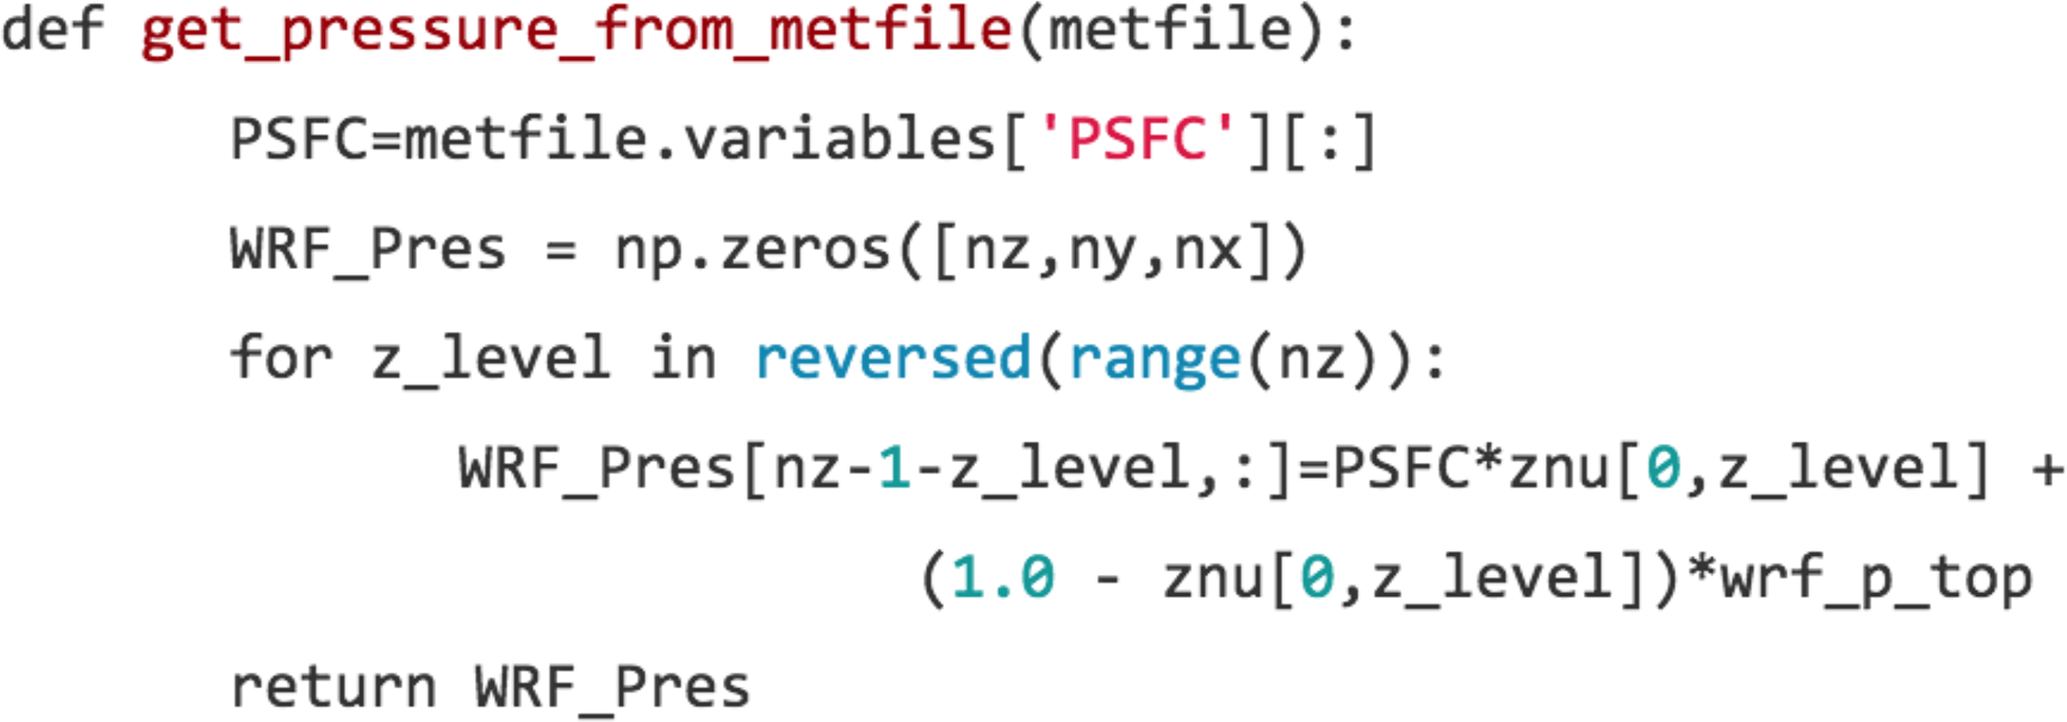
\includegraphics[width=10cm]{f1.png}
\caption{A Python script, which reconstructs the pressure using the \textit{met\_em\_...*} files. nx, ny, and nz indicate the number of grid nodes in WRF-Chem domain.}
\label{fig:figA1}
\end{figure}

\subsection{Mapping chemical species between MERRA-2 and WRF-Chem}

{Merra2BC} file \textit{config.py} contains multiplication factors to convert MERRA-2 mass mixing ratios of gases given in kg\,kg$^{-1}$ into \unit{ppmv}. Aerosols are converted from kg\,kg$^{-1}$ to \unit{\mu}g\,kg$^{-1}$. When using the GOCART aerosol module in WRF-Chem simulation, all MERRA-2 aerosols and gases are matched with those from WRF-Chem. We simply multiply by a factor of $10^9$ to convert MERRA-2 aerosol mixing ratios given in kg\,kg$^{-1}$ into \unit{\mu}g\,kg$^{-1}$. In the case of gases, we need to multiply MERRA-2 mass mixing ratios by a ratio of molar masses $M_{air}/M_{gas}$ multiplied by $10^6$ to convert kg\,kg$^{-1}$ into \unit{ppmv}, where $M_{gas}$ and $M_{air}$ are molar masses (g\,mol$^{-1}$) of the required gas and air (28.97\,g\,mol$^{-1}$), respectively. If another aerosol module is chosen in WRF-Chem, then different multiplication factors should be used.

\subsection{Interpolation procedure}

A brief description of the interpolation procedure applied to the initial conditions is presented in Alg.~\ref{fig:figA2}. For boundary conditions, the procedure is similar, except that additional updates of domain boundary tendencies are required and interpolation is performed for each step, where boundary conditions are applied.

\begin{algorithm}
\caption{Interpolation procedure applied to initial conditions.}
\label{fig:figA2}
\begin{algorithmic}[1]
    \State Pressure reconstruction at each node of the MERRA-2 and WRF-Chem grids.
    \Statex
    \For {each 72 vertical layers in MERRA-2 grid}
\State \multiline{%
Horizontal interpolation of MERRA-2 pressure on WRF-Chem latitude, longitude nodes using bivariate spline approximation (method $RectBivariateSpline$ from Scipy module).}

	\EndFor
	\State \textbf{Result}: MERRA-2 pressure is calculated on 72 levels but on latitude, longitude nodes of the WRF-Chem grid.
    \Statex
    \For {each chemical species mixing ratio}
        \For{each 72 vertical layers in MERRA-2 grid}
            \State \multiline{%
            Horizontal interpolation of MERRA-2 species mixing ratio on WRF-Chem latitude, longitude nodes using bivariate spline approximation (method $RectBivariateSpline$ from Scipy module).}
        \EndFor
        \State \multiline{%
        \textbf{Result}: MERRA-2 species mixing ratio is calculated on 72 levels but on latitude, longitude nodes of WRF-Chem grid.}
        \Statex
        \Statex
        \For{each lat, long node of the WRF-Chem grid}
            \State \multiline{%
            Vertical linear interpolation of MERRA-2 species mixing ratio on WRF-Chem vertical coordinate (method $interp1d$ from from Scipy module). }
        \EndFor
        \State \multiline{%
        \textbf{Result}: MERRA-2 species mixing ratio is interpolated at each node of WRF-Chem grid.}
        \Statex
        \Statex
        \State \multiline{%
        Multiplying interpolated species mixing ratio by corresponding factor to convert kg\,kg$^{-1}$ into \unit{ppmv} or \unit{\mu}g\,kg$^{-1}$, depending whether it gas or aerosol.}
        
        \State \multiline{%
        Updating corresponding fields in WRF-Chem $wrfinput\_d01$ file by interpolated values.}
	\EndFor
	\State \textbf{Result}: WRF-Chem grid is updated by interpolated values from MERRA-2 grid.
\end{algorithmic}
\end{algorithm}

\subsection{Typical workflow}

Here are the steps describing how to work with the {Merra2BC} interpolator:
\begin{enumerate}
\item Run \textit{real.exe}, which will produce initial \textit{wrfinput\_d01} and boundary conditions \textit{wrfbdy\_d01} files required by the WRF-Chem simulation.
\item Download required MERRA-2 files from \url{https://disc.gsfc.nasa.gov/daac-bin/FTPSubset2.pl};
\item Download {Merra2BC} from \url{https://github.com/saneku/Merra2BC}.
\item Edit the \textit{config.py} file which contains
\begin{itemize}
\item[a.] mapping of chemical species and aerosols between MERRA-2 and WRF-Chem;
\item[b.] paths to \textit{wrfinput\_d01}, \textit{wrfbdy\_d01}, and \textit{met\_em\_...*} files;
\item[c.] a path to the downloaded MERRA-2 files.
\end{itemize}
\item \textit{real.exe} sets default boundary and initial conditions for some chemical species.  {Merra2BC} adds interpolated values to the existing values, which may cause incorrect concentration values. To avoid this, run ``python \textit{zero\_fileds.py}'', which will zero the required fields.
\item Run ``python \textit{main.py}'', which will do the interpolation. As a result, files \textit{wrfinput\_d01} and \textit{wrfbdy\_d01} will be updated by the interpolated from MERRA-2 values.
\item Modify the WRF-Chem \textit{namelist.input} file at section \textit{\&chem}: set \textit{have\_bcs\_chem = .true.} to activate updated boundary conditions and, if needed, \textit{chem\_in\_opt = 1} to activate updated initial conditions.
\item Run \textit{wrf.exe}.
\end{enumerate}

\section{How to cite}
If you find this code useful in your research, please consider citing:

\hack{\newpage}
\bibliographystyle{plain}

\bibliography{references}
\end{document}
